\documentclass[aspectratio=169,11pt]{beamer}

\usepackage[utf8]{inputenc}
\usepackage[T1]{fontenc}
\usepackage{booktabs}
\usepackage{tikz}
\usepackage{pgfplots}
\pgfplotsset{compat=1.16}
\usetikzlibrary{arrows.meta,positioning,shapes.geometric}

\usetheme{Madrid}
\usecolortheme{seahorse}
\setbeamertemplate{navigation symbols}{}
\setbeamertemplate{footline}[frame number]
% Plain glyph bullets: the default shaded ball bullets render only once in some PDF viewers.
\setbeamertemplate{itemize item}{\color{structure}$\bullet$}
\setbeamertemplate{itemize subitem}{\color{structure}$\circ$}

\newcommand{\m}[1]{\texttt{\detokenize{#1}}}
\definecolor{good}{RGB}{34,139,34}
\definecolor{bad}{RGB}{200,40,40}
\newcommand{\good}[1]{\textcolor{good}{\textbf{#1}}}
\newcommand{\bad}[1]{\textcolor{bad}{\textbf{#1}}}

\title{Adaptive tracing and trace reduction}
\subtitle{How much can we drop without losing the anomalies?}
\author{Joonas}
\institute{CS-E4660 course project}
\date{November 2026}

\begin{document}

\begin{frame}
  \titlepage
\end{frame}

% ------------------------------------------------------------------
\begin{frame}{Research questions}
  \begin{itemize}
    \item Is it worth going deeper than OpenTelemetry collector config options for trace processing?
    \item Do simple reducers miss rare exceptions?
    \item Does a smarter reducer matter enough for finding exceptions and anomalies?
    \item Application-level vs.\ collector-level adaptability?
    \item Can an LLM keep up at reasonable cost? \hfill \textit{(not tested)}
  \end{itemize}
\end{frame}

% ------------------------------------------------------------------
\begin{frame}{Case study: a workload with a ground truth}
  Production traces have no ground truth: nobody knows which trace held the problem.
  \medskip

  \begin{columns}[T]
    \begin{column}{0.55\textwidth}
      \textbf{Mock data platform} (Dagster + OpenTelemetry)
      \begin{itemize}
        \item 49 jobs: importers, transformers, loaders
        \item IO operations mocked with descriptive names and trace metadata: DB, cloud storage, HTTP, first- and third-party services
        \item $\approx$900 spans per trace, jobs in their own processes
        \item Overlapping runs, seeded and repeatable
      \end{itemize}
    \end{column}
    \begin{column}{0.45\textwidth}
      \textbf{Injected, labelled anomalies}
      \begin{itemize}
        \item rare slow service calls (20--30$\times$)
        \item huge uploads
        \item outage windows, background failures
        \item every anomaly logged by trace and span ID, independent of what any collector keeps
      \end{itemize}
    \end{column}
  \end{columns}
\end{frame}

% ------------------------------------------------------------------
\begin{frame}{Methods under test}
  \footnotesize
  \begin{tabular}{@{}lll@{}}
    \toprule
    Group & Methods & Holds \\
    \midrule
    Reference & \m{baseline_naive} & keeps everything \\
    Stock, stateless & \m{sampling} (10\% of traces) & nothing \\
    Stock, tail sampling & \m{anomalies_sampling}, \m{anomalies_sampling_limited}, & whole traces \\
     & \m{routed_tail_sampling} (per-job hold 45--90\,s) & until decision \\
    Calibrated collector & \m{span_filter} & nothing \\
    Application side & \m{job_buffer}, \m{resolution} & a job, or nothing \\
    LLM agent & --- (no time) & \\
    \bottomrule
  \end{tabular}

  \bigskip
  \small
  \m{span_filter} and \m{routed_tail_sampling} are plain collector configuration, generated from thresholds learned on a baseline run (5$\times$ the median duration per service and span name).
  All methods decide on errors and durations only, never on the labels.
\end{frame}

% ------------------------------------------------------------------
\begin{frame}{Metrics and experiment design}
  \begin{columns}[T]
    \begin{column}{0.5\textwidth}
      \textbf{Metrics}
      \begin{itemize}
        \item \textbf{Reduction}: traces, spans, bytes kept
        \item \textbf{Evidence}: anomalous traces where a span with an injected anomaly was kept
        \item Recall by trace type (normal traces show waste)
        \item \textbf{Cost}: peak collector memory, OOM kills, refused requests
      \end{itemize}
      Trace-level recall hides what span-level methods lose: they keep a skeleton of every trace.
    \end{column}
    \begin{column}{0.5\textwidth}
      \textbf{Design}
      \begin{itemize}
        \item \textbf{Accuracy}: 260 live runs at 0.5/s, all collectors fed the same spans
        \item \textbf{Out of sample}: calibrated on seed 42, tested on 7, 8, 9
        \item \textbf{Scale}: replay of a recorded capture at 5--40 traces/s, each collector alone in Docker
        \item \textbf{Drift}: latencies $\times$0.5 and $\times$2
      \end{itemize}
    \end{column}
  \end{columns}

\end{frame}

% ------------------------------------------------------------------
\begin{frame}{How a run is scored}
  \centering
  \vspace{6mm}
  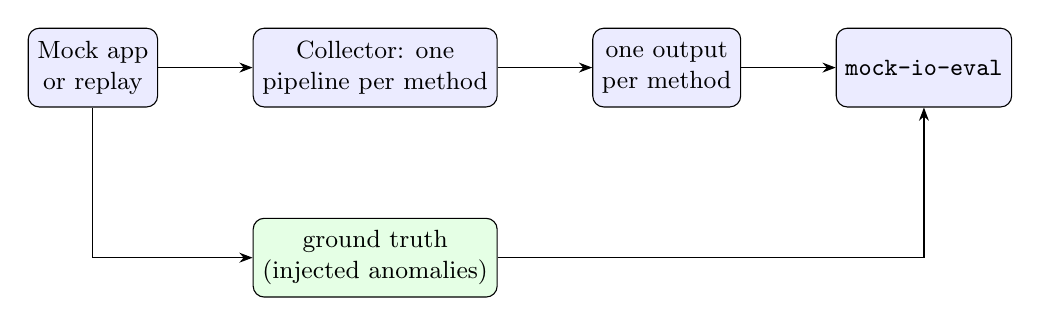
\begin{tikzpicture}[node distance=12mm, every node/.style={font=\small},
      box/.style={draw, rounded corners, minimum height=10mm, fill=blue!8, align=center},
      >={Stealth}]
    \node[box] (app) {Mock app\\ or replay};
    \node[box, right=of app] (col) {Collector: one\\ pipeline per method};
    \node[box, right=of col] (out) {one output\\ per method};
    \node[box, right=of out] (eval) {\m{mock-io-eval}};
    \node[box, below=14mm of col, fill=green!10] (gt) {ground truth\\ (injected anomalies)};
    \draw[->] (app) -- (col);
    \draw[->] (col) -- (out);
    \draw[->] (out) -- (eval);
    \draw[->] (app) |- (gt);
    \draw[->] (gt) -| (eval);
  \end{tikzpicture}

  \bigskip
  \small
  Every method sees the same spans at the same time, so methods are compared on identical traces.
  The ground truth is written by the app, independent of what any collector keeps.
\end{frame}

% ------------------------------------------------------------------
\begin{frame}{Result 1: calibrated span-level methods keep the evidence}
  \centering
  \begin{tikzpicture}
    \begin{axis}[
        ybar, bar width=7pt, width=0.95\textwidth, height=0.58\textheight,
        ymin=0, ymax=110, ylabel={share kept (\%)},
        symbolic x coords={a,b,c,d,e,f,g},
        xtick=data, xticklabels={\m{sampling}, \m{anomalies_sampling}, \m{anomalies_sampling_limited}, \m{routed_tail_sampling}, \m{span_filter}, \m{app_job_buffer}, \m{app_resolution}}, x tick label style={rotate=20, anchor=east, font=\scriptsize},
        legend style={at={(0.5,1.05)}, anchor=south, legend columns=2, font=\footnotesize},
        enlarge x limits=0.08, nodes near coords, every node near coord/.append style={font=\tiny},
      ]
      \addplot[fill=gray!60] coordinates {(a,10.3) (b,100) (c,38.3) (d,37.0) (e,15.0) (f,40.6) (g,14.5)};
      \addplot[fill=blue!60] coordinates {(a,14.5) (b,100) (c,44.6) (d,47.0) (e,100) (f,100) (g,100)};
      \legend{spans kept, evidence}
    \end{axis}
  \end{tikzpicture}

  {\footnotesize Live run, seed 8 (out of sample); seed 7 is similar. \m{anomalies_sampling} keeps everything: its 1\,s policy matches almost every trace.}
\end{frame}

% ------------------------------------------------------------------
\begin{frame}{Result 2: tail sampling runs out of memory}
  \begin{columns}[T]
    \begin{column}{0.55\textwidth}
      \begin{tikzpicture}
        \begin{axis}[
            width=\textwidth, height=0.5\textheight,
            xlabel={traces/s}, ylabel={peak memory (MB)},
            xmode=log, log basis x=2, xtick={5,10,20,40}, xticklabels={5,10,20,40},
            legend pos=north west, legend style={font=\scriptsize}, grid=major,
          ]
          \addplot[color=red, mark=square*] coordinates {(5,245) (10,443) (20,847) (40,1557)};
          \addplot[color=orange, mark=triangle*] coordinates {(5,159) (10,262) (20,392) (40,1079)};
          \addplot[color=green!50!black, mark=*] coordinates {(5,104) (10,110) (20,113) (40,124)};
          \legend{\m{routed_tail_sampling}, \m{anomalies_sampling}, \m{span_filter}}
        \end{axis}
      \end{tikzpicture}

      {\scriptsize 5\,s hold, no limit, replay.}
    \end{column}
    \begin{column}{0.45\textwidth}
      With realistic \textbf{90\,s holds} and a 1\,GB limit:
      \begin{itemize}
        \item \m{anomalies_sampling}: at the limit already at 5/s, \bad{killed at 10/s}
        \item \m{routed_tail_sampling}: 698\,MB at 5/s, \bad{killed at 10/s}
        \item \m{span_filter}: \good{110--117\,MB}, 100\% evidence
      \end{itemize}
      \smallskip
      Memory $\propto$ rate $\times$ hold time, and an OOM loses everything held, not just the excess.
    \end{column}
  \end{columns}
\end{frame}

% ------------------------------------------------------------------
\begin{frame}{Result 3: whole-trace latency cannot find the anomalies}
  \m{routed_tail_sampling} kept only 47\% of the evidence, even with a full flush.
  All 44 missed anomalous traces were fully routed single-job traces under their job's slow threshold.

  \medskip
  \begin{columns}[T]
    \begin{column}{0.5\textwidth}
      Trace duration relative to the job's threshold: anomalous median \textbf{78\%}, normal median \textbf{70\%}.
      \medskip

      \small
      \begin{tabular}{@{}rrr@{}}
        \toprule
        cutoff (\% of thr.) & anomalies caught & normal kept \\
        \midrule
        100 & 17\% & 13\% \\
        80  & 43\% & 29\% \\
        60  & 94\% & 75\% \\
        50  & 100\% & 95\% \\
        \bottomrule
      \end{tabular}
    \end{column}
    \begin{column}{0.5\textwidth}
      \begin{itemize}
        \item Any cutoff that finds the anomalies keeps nearly every normal trace.
        \item The collector's tail-sampling latency policy only sees \textbf{whole-trace} duration.
        \item The injected slow span stands out on its own, which is why the span-level methods work.
      \end{itemize}
    \end{column}
  \end{columns}
\end{frame}

% ------------------------------------------------------------------
\begin{frame}{Result 4: the span-level methods hold up}
  \small
  \begin{tabular}{@{}lrrrrr@{}}
    \toprule
    Method & spans kept & evidence & slow recall & normal traces kept & collector MB \\
    \midrule
    \m{span_filter} & 15\% & 100\% & 100\% & 100\% & 104--125 \\
    \m{app_resolution} & 14\% & 100\% & 100\% & 100\% & 62--90 \\
    \m{app_job_buffer} & 24--41\% & 100\% & 94--100\% & 29--42\% & 84--139 \\
    \bottomrule
  \end{tabular}

  \medskip
  \begin{itemize}
    \item Replayed at 5--40 traces/s on two seeds, and on a capture the thresholds never saw: reduction and memory stay \textbf{flat with rate}.
    \item App-side rules are emulated in the replay; on a live capture the emulation keeps exactly the same spans as the real processors (31,920 and 89,487 of 220,354).
    \item \m{app_job_buffer} drops whole traces and its reduction depends on the capture.
    \item Not measured: the CPU and memory the reducers cost \emph{inside} the app.
  \end{itemize}
\end{frame}

% ------------------------------------------------------------------
\begin{frame}{Robustness: latency drift}
  Thresholds stay calibrated at normal latency; the workload runs at half and double speed.

  \medskip
  \centering
  \begin{tabular}{llrrr}
    \toprule
    latency & method & spans kept & evidence & normal traces kept \\
    \midrule
    $\times$0.5 & \m{span_filter}     & 15.0\% & 98.9\% & 100\% \\
    $\times$0.5 & \m{app_resolution}  & 14.1\% & 97.8\% & 100\% \\
    $\times$0.5 & \m{app_job_buffer}  & 39.2\% & 97.8\% & 34\% \\
    $\times$2   & \m{span_filter}     & 15.5\% & 100\% & 100\% \\
    $\times$2   & \m{app_resolution}  & 17.3\% & 100\% & 100\% \\
    $\times$2   & \m{app_job_buffer}  & \bad{92.2\%} & 100\% & 97\% \\
    \bottomrule
  \end{tabular}

  \medskip
  \raggedright\small
  Faster than calibrated: first small evidence misses. Slower: evidence holds, but \m{app_job_buffer}'s reduction disappears (a part is kept if any span is slow).
  Recalibrate on a recent baseline when the workload changes. One run per scale.
\end{frame}

% ------------------------------------------------------------------
\begin{frame}{Answers to the research questions}
  \small
  \begin{description}
    \item[Beyond collector config?] \textbf{Partly.} The best collector method is still plain config, but generated from calibrated thresholds. The stock tail-sampling configs failed. What pays off is calibrated, span-level decisions, not custom code.
    \item[Simple reducers miss rare exceptions?] \textbf{Yes.} 10\% sampling keeps 13--15\% of the evidence; some anomaly types are missed completely.
    \item[Smarter reducer worth it?] \textbf{Yes, for calibrated span-level thresholds}: 100\% evidence at 15\% of the spans. Not tested for an LLM-based reducer.
    \item[LLM at reasonable cost?] \textbf{Not tested.}
    \item[Application vs.\ collector?] \textbf{Some advantages in the app}: it knows when a job ends and \m{resolution} keeps the fewest spans. But \m{span_filter} reaches the same evidence without touching the app, \m{job_buffer} is the most drift-sensitive, and the in-app cost is unmeasured.
  \end{description}
\end{frame}

% ------------------------------------------------------------------
\begin{frame}{Lessons and limitations}
  \begin{columns}[T]
    \begin{column}{0.52\textwidth}
      \textbf{Lessons}
      \begin{itemize}
        \item Decide on the span, not the trace.
        \item Hold nothing where possible: memory is rate $\times$ hold time.
        \item Calibrate on a recent baseline; drift matters.
        \item Measure against a ground truth; trace-level recall hides losses.
        \item Mocking and a single laptop limit scale, a compute cluster would have taken more time than available.
      \end{itemize}
    \end{column}
    \begin{column}{0.48\textwidth}
      \textbf{Limitations}
      \begin{itemize}
        \item One synthetic workload; no real production traces
        \item Mock app too slow for high rates, so replay is used for scale
        \item LLM agent was not tested
        \item In-app cost of reducers unmeasured
        \item Mostly one run per setting
      \end{itemize}
      \smallskip
    \end{column}
  \end{columns}
\end{frame}

\end{document}
